\section{Análisis de Sentimientos}

\subsection{Metodología}

\begin{figure}[H]
    \center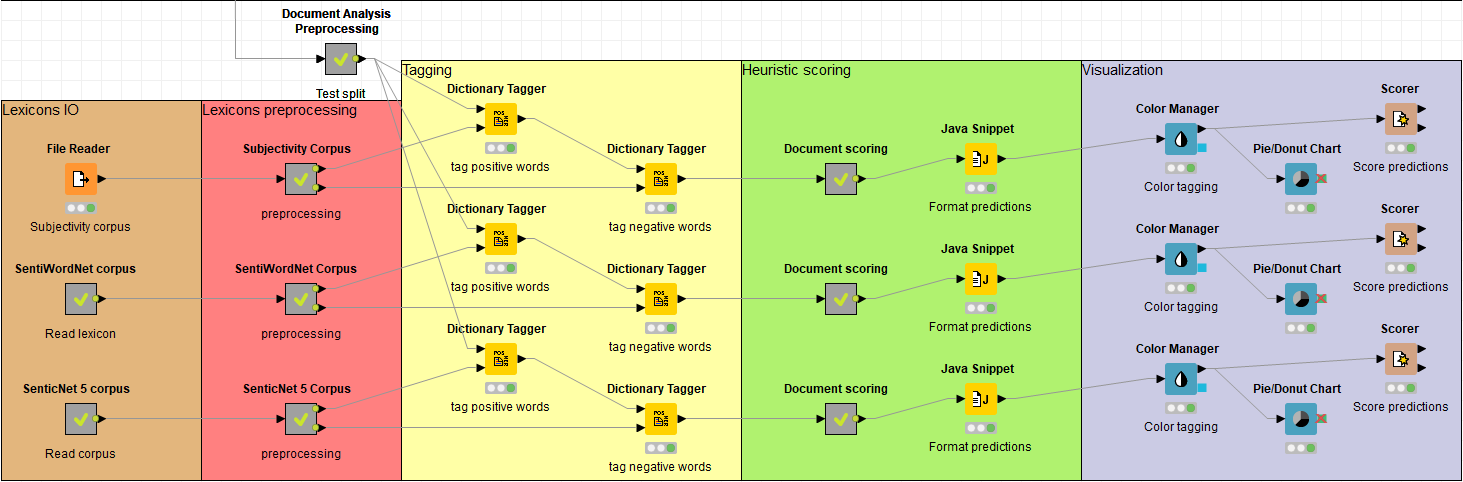
\includegraphics[width=.95\linewidth]{img/analysis/workflow.png}
    \caption{Workflow general del análisis de sentimientos.}
\end{figure}

Para hacer una comparativa justa de resultados, se aplica el análisis de sentimientos a la misma partición de test con la que se evalúan los métodos de clasificación.

Como preprocesamiento de los documentos aplicamos un Parts Of Speech tagging y Stanford Lemmatizer para quitar las inflexiones de las palabras.

\vspace{\baselineskip}

Por otro lado, la lectura de los lexicon varía con cada uno:
\begin{itemize}
    \item Para el corpus MPQA se usa el mismo procedimiento proporcionado en clase.
    \item Para SentiWordNet, puesto que cada synterm puede contener más de una palabra, estas se separan en nuevas fila con los mismos valores de sentimiento.
    \vspace{\baselineskip}
    Seguidamente calculamos el valor de objetividad como $1 - (POS + NEG)$ y a cada término le asignamos un valor \textbf{neutral} si ambos \textit{PosScore} y \textit{NegScore} son iguales, en otro caso se le asigna la etiqueta con el score más alto.
    \vspace{\baselineskip}
    Por último agrupamos las filas dónde coincidan el synterm, de forma que no se etiqueten algunas palabras con sentimientos diferentes. Para ello hacemos uso del nodo \textit{Group By} y asignamos el sentimiento y el valor de objetividad en base a la moda y a la media respectivamente.
    \item Para SenticNet modificamos el delimitador de columna por uno nuevo, y le asociamos a cada término el valor de \textbf{polarity} indicado.
\end{itemize}

\begin{figure}[H]
    \center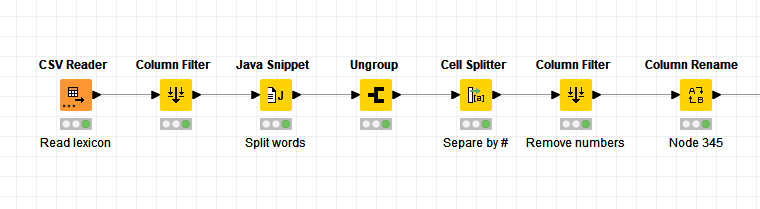
\includegraphics[width=.95\linewidth]{img/analysis/sentiword-reading.png}
    \caption{Lectura del lexicon SentiWordNet.}
\end{figure}

\begin{figure}[H]
    \center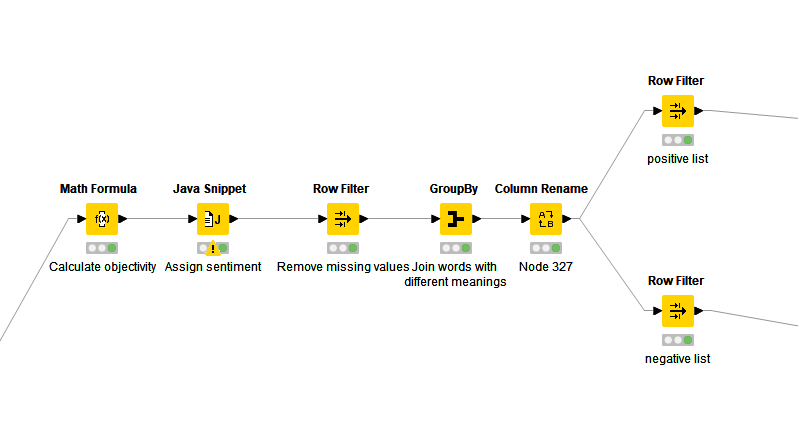
\includegraphics[width=.95\linewidth]{img/analysis/sentiword-prepro.png}
    \caption{Preprocesamiento del lexicon SentiWordNet.}
\end{figure}

\begin{figure}[H]
    \center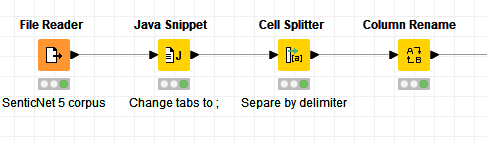
\includegraphics[width=.95\linewidth]{img/analysis/senticnet-reading.png}
    \caption{Lectura del lexicon SenticNet.}
\end{figure}

Finalmente asignamos a cada documento el sentimiento en base al mayor número de palabras que tenga de uno u otro.

% -----------

\subsection{Resultados}

\begin{figure}[H]
    \center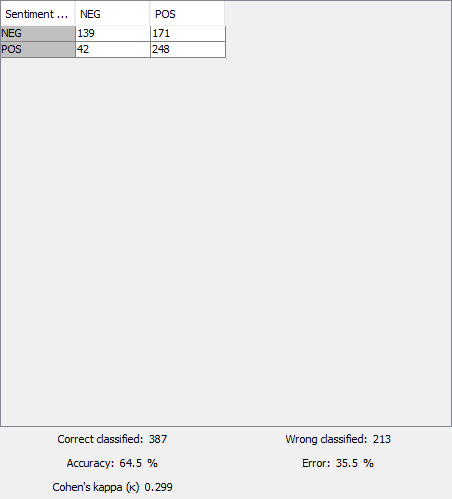
\includegraphics[width=.95\linewidth]{img/analysis/score1.png}
    \caption{Matriz de confusión con MPQA.}
\end{figure}

\begin{figure}[H]
    \center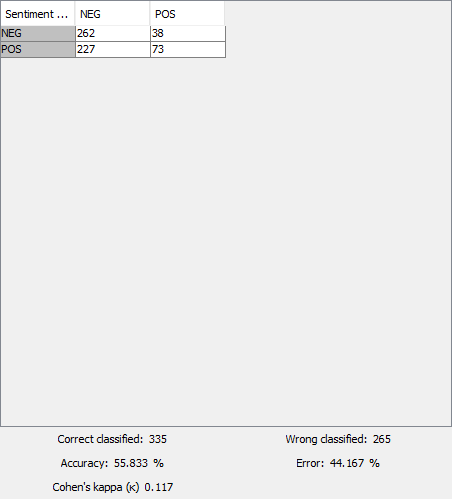
\includegraphics[width=.95\linewidth]{img/analysis/score2.png}
    \caption{Matriz de confusión con SentiWordNet.}
\end{figure}

\begin{figure}[H]
    \center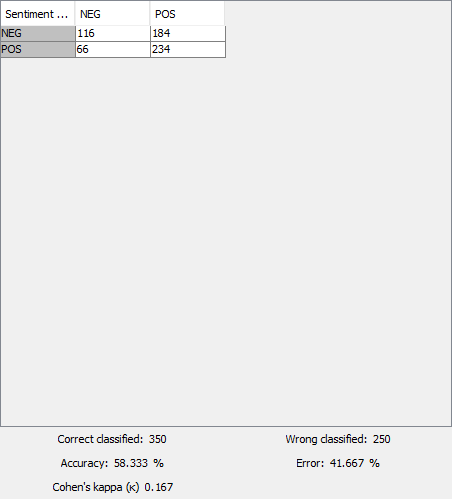
\includegraphics[width=.95\linewidth]{img/analysis/score3.png}
    \caption{Matriz de confusión con SenticNet.}
\end{figure}

\newpage

\begin{figure}[H]
    \center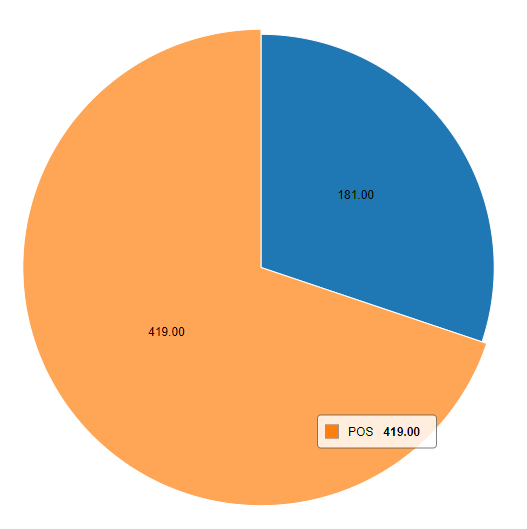
\includegraphics[height=.4\linewidth]{img/analysis/pie1.png}
    \caption{Pie chart con MPQA.}
\end{figure}

\begin{figure}[H]
    \center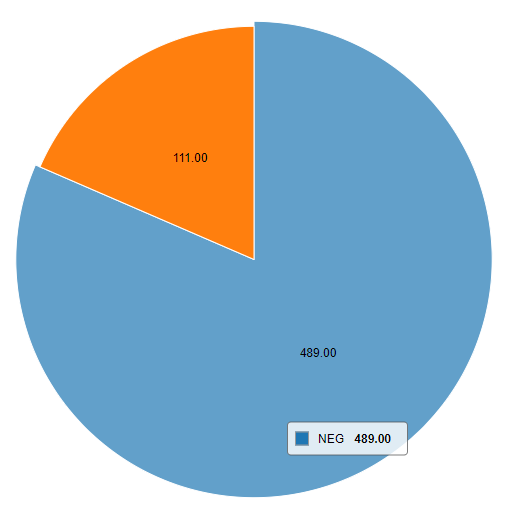
\includegraphics[height=.4\linewidth]{img/analysis/pie2.png}
    \caption{Pie chart con SentiWordNet.}
\end{figure}

\begin{figure}[H]
    \center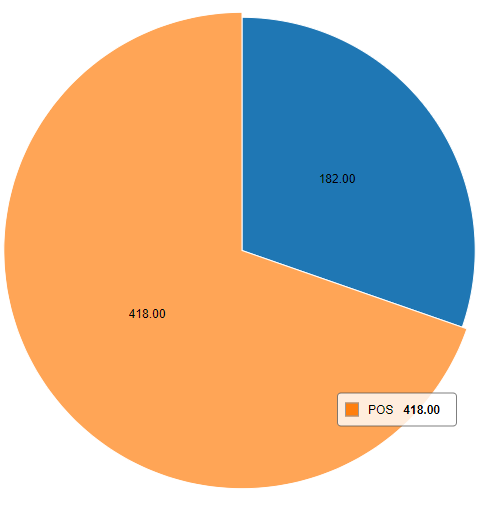
\includegraphics[height=.4\linewidth]{img/analysis/pie3.png}
    \caption{Pie chart con SenticNet.}
\end{figure}